% =============================================================================
% MUSAS documentation -- user guide and API reference
% Build: latexmk -lualatex -shell-escape musas_documentation.tex   (or: make pdf)
% The listings of chapters 3 and 4 are read from snippets/, the same files used
% to build getting_started.ipynb (tools/build_notebook.py).
% =============================================================================
\documentclass[11pt,a4paper,oneside]{report}

% ----------------------------------------------------------------------------
% Fonts, page, colours
% ----------------------------------------------------------------------------
\usepackage{fontspec}
\setmainfont{Lato}
\setmonofont{JetBrains Mono}[Scale=0.84]
\usepackage[a4paper,left=2.5cm,right=2.5cm,top=2.7cm,bottom=2.6cm,
            headheight=14pt]{geometry}
\usepackage{xcolor}
\definecolor{primary}{HTML}{002D4D}
\definecolor{primarylight}{HTML}{E6EEF4}
\definecolor{accent}{HTML}{E8637D}
\definecolor{accentlight}{HTML}{FCEEF1}
\definecolor{mint}{HTML}{2E9C7A}
\definecolor{mintlight}{HTML}{EAF8F2}
\definecolor{amber}{HTML}{C9781E}
\definecolor{amberlight}{HTML}{FDF3E6}
\definecolor{ink}{HTML}{1F2933}
\definecolor{muted}{HTML}{66788A}
\definecolor{codebg}{HTML}{F6F8FA}
\definecolor{codeframe}{HTML}{D5DEE6}
\color{ink}

\usepackage{graphicx}
\usepackage{booktabs}
\usepackage{array}
\usepackage{tabularx}
\usepackage{longtable}
\usepackage{enumitem}
\usepackage{fontawesome5}
\usepackage{tikz}
\usetikzlibrary{arrows.meta,calc,positioning}
% Shared style of the sequence diagrams of the simple experiments.
% Solid arrows are network messages; dashed arrows are internal calls.
\definecolor{seqmsg}{HTML}{D9822B}
\definecolor{sequas}{HTML}{D9D9D9}
\definecolor{sequtm}{HTML}{CFE3C3}
\definecolor{seqenv}{HTML}{CFE0EE}
\definecolor{seqtime}{HTML}{DCE8F4}
\tikzset{
    seq/.style={x=1cm, y=1cm, font=\footnotesize},
    seqlane/.style={draw=black!55, rounded corners=6pt, minimum height=0.8cm,
        text width=2.2cm, align=center, font=\small, inner sep=2pt},
    sequas/.style={seqlane, fill=sequas},
    sequtm/.style={seqlane, fill=sequtm},
    seqenv/.style={seqlane, fill=seqenv},
    seqline/.style={black!70, line width=1.1pt, dash pattern=on 7pt off 4pt},
    seqguide/.style={black!25, line width=0.4pt, densely dotted},
    seqmsg/.style={-{Stealth[length=2.4mm, width=1.8mm]}, line width=0.9pt,
        color=seqmsg},
    seqcall/.style={seqmsg, dash pattern=on 3pt off 2pt},
    seqlbl/.style={align=center, font=\scriptsize, inner sep=1.5pt, text=black!85,
        fill=white, fill opacity=0.9, text opacity=1},
    seqnote/.style={draw=black!45, fill=white, rounded corners=2pt,
        align=center, font=\scriptsize, inner sep=2.5pt},
    seqtick/.style={font=\scriptsize, inner sep=1pt},
    seqmark/.style={circle, fill=black!70, inner sep=0pt, minimum size=5pt},
}
% \seqtimearrow{x start}{x end}{y}
\newcommand{\seqtimearrow}[3]{%
    \fill[seqtime, draw=black!45] (#1,#3+0.22) -- (#2-0.5,#3+0.22)
        -- (#2-0.5,#3+0.42) -- (#2,#3) -- (#2-0.5,#3-0.42)
        -- (#2-0.5,#3-0.22) -- (#1,#3-0.22) -- cycle;
    \node[font=\small] at ({(#1+#2)/2},#3) {Simulated time};
}

\usepackage[most,minted]{tcolorbox}
\setminted{fontsize=\small, breaklines, style=friendly}
\usepackage{titlesec}
\usepackage{fancyhdr}
\usepackage{caption}
\captionsetup{font={small,color=muted}, labelfont={bf,color=primary}}
\usepackage[hidelinks]{hyperref}
\hypersetup{colorlinks, linkcolor=primary, urlcolor=accent,
  pdftitle={MUSAS Documentation}, pdfauthor={Caio Bianchi}}

\setlength{\parindent}{0pt}
\setlength{\emergencystretch}{2.5em}
\setlength{\parskip}{0.55em}
\setlist{itemsep=0.15em, topsep=0.3em}
\setlist[itemize]{label={\color{accent}\small\textbullet}}
\newcolumntype{L}[1]{>{\raggedright\arraybackslash}p{#1}}
\newcolumntype{Y}{>{\raggedright\arraybackslash}X}
\renewcommand{\arraystretch}{1.18}

% ----------------------------------------------------------------------------
% Headings
% ----------------------------------------------------------------------------
\titleformat{\chapter}[display]
  {\color{primary}\bfseries}
  {\begin{tikzpicture}
     \node[fill=accent, text=white, minimum size=1.1cm, rounded corners=3pt,
           font=\huge\bfseries] {\thechapter};
   \end{tikzpicture}}
  {0.6em}
  {\Huge}
  [\vspace{0.4em}{\color{codeframe}\titlerule[1.2pt]}]
\titlespacing*{\chapter}{0pt}{-10pt}{22pt}
\titleformat{\section}
  {\color{primary}\Large\bfseries}{\color{accent}\thesection}{0.8em}{}
\titleformat{\subsection}
  {\color{primary}\large\bfseries}{\color{accent}\thesubsection}{0.8em}{}
\titleformat{\subsubsection}
  {\color{primary}\normalsize\bfseries}{}{0em}{}
\titlespacing*{\section}{0pt}{1.4em}{0.5em}
\titlespacing*{\subsection}{0pt}{1.1em}{0.35em}
\setcounter{secnumdepth}{2}
\setcounter{tocdepth}{1}

\pagestyle{fancy}
\fancyhf{}
\fancyhead[L]{\small\color{muted}\textbf{MUSAS} Documentation}
\fancyhead[R]{\small\color{muted}\leftmark}
\fancyfoot[C]{\small\color{primary}\thepage}
\renewcommand{\headrulewidth}{0.4pt}
\renewcommand{\headrule}{{\color{codeframe}\hrule height\headrulewidth}}
\renewcommand{\chaptermark}[1]{\markboth{#1}{}}
\fancypagestyle{plain}{\fancyhf{}\fancyfoot[C]{\small\color{primary}\thepage}%
  \renewcommand{\headrulewidth}{0pt}}

% ----------------------------------------------------------------------------
% Boxes
% ----------------------------------------------------------------------------
\tcbset{
  codestyle/.style={enhanced, breakable, colback=codebg, colframe=codeframe,
    boxrule=0.5pt, arc=3pt, left=6pt, right=6pt, top=3pt, bottom=3pt,
    fonttitle=\footnotesize\ttfamily, coltitle=muted,
    attach boxed title to top right={yshift=-2.2mm, xshift=-3mm},
    boxed title style={colback=white, colframe=codeframe, boxrule=0.5pt,
      arc=2pt, top=0pt, bottom=0pt, left=3pt, right=3pt}},
}
% listing read from snippets/ (identical to the notebook cell)
\newtcbinputlisting{\snippet}[1]{codestyle, listing only,
  listing engine=minted, minted language=python,
  listing file={snippets/#1}, title={\faBook\ notebook: \detokenize{#1}}}
% printed output of a snippet
\newtcbinputlisting{\snippetoutput}[1]{enhanced, breakable, listing only,
  listing engine=minted, minted language=text,
  minted options={fontsize=\footnotesize, breaklines},
  listing file={snippets/output/#1}, colback=primary, colupper=white,
  colframe=primary, boxrule=0pt, arc=3pt, left=6pt, top=2pt, bottom=2pt,
  title={\faTerminal\ output}, fonttitle=\footnotesize\bfseries,
  coltitle=white, colbacktitle=primary!80!black, toptitle=0pt,
  bottomtitle=0pt}
% inline Python and shell examples
\newtcblisting{pycode}{codestyle, listing only, listing engine=minted,
  minted language=python}
\newtcblisting{shell}{codestyle, listing only, listing engine=minted,
  minted language=bash, colback=primarylight}

% callouts
\newtcolorbox{callout}[4]{enhanced, breakable, colback=#2, colframe=#1,
  boxrule=0pt, leftrule=3pt, arc=0pt, outer arc=0pt, left=8pt,
  top=4pt, bottom=4pt, before upper={{\color{#1}#3\ \textbf{#4}}\quad}}
\newenvironment{tip}{\begin{callout}{mint}{mintlight}{\faLightbulb[regular]}{Tip.}}{\end{callout}}
\newenvironment{note}{\begin{callout}{primary}{primarylight}{\faInfoCircle}{Note.}}{\end{callout}}
\newenvironment{warning}{\begin{callout}{accent}{accentlight}{\faExclamationTriangle}{Attention.}}{\end{callout}}

% API entries
\newtcolorbox{api}[2]{enhanced, breakable, colback=white, colframe=codeframe,
  boxrule=0.6pt, arc=3pt, left=8pt, right=8pt, top=4pt, bottom=4pt,
  colbacktitle=primarylight, coltitle=primary, fonttitle=\bfseries,
  title={\ttfamily #1\hfill\normalfont\footnotesize\color{muted}#2},
  before skip=0.9em, after skip=0.9em}
\newcommand{\sig}[1]{\par{\small\ttfamily\def\_{\textunderscore\allowbreak}\color{primary!85!black}#1}\par}
\newenvironment{params}[1][Parameters]
  {\par\smallskip{\footnotesize\bfseries\color{muted}\MakeUppercase{#1}}\par
   \begin{description}[font=\normalfont, leftmargin=1.2em, labelindent=0pt,
     itemsep=0.25em, style=nextline]}
  {\end{description}}
\newcommand{\p}[3]{\item[{\ttfamily\color{primary}\bfseries #1}%
  {\ \footnotesize\color{muted}\ttfamily #2}] #3}
\newcommand{\returns}[1]{\par{\footnotesize\bfseries\color{muted}RETURNS}\quad #1\par}
\newcommand{\code}[1]{\textcolor{primary!85!black}{\ttfamily\def\_{\textunderscore\allowbreak}#1}}
\newcommand{\pkg}[1]{\textcolor{accent!85!black}{\ttfamily #1}}

% ----------------------------------------------------------------------------
\begin{document}

% =============================================================================
% COVER
% =============================================================================
\begin{titlepage}
\begin{tikzpicture}[remember picture, overlay]
  \fill[primary] (current page.north west) rectangle
    ([yshift=10.5cm]current page.south east);
  \fill[accent] ([yshift=10.5cm]current page.south west) rectangle
    ([yshift=10.2cm]current page.south east);
  % stylised traffic: dashed routes and UAS markers
  \begin{scope}[shift={([xshift=12.2cm, yshift=-8.6cm]current page.north west)},
                opacity=0.9]
    \foreach \a/\c in {0/white, 35/white!70!primary, 70/white!50!primary,
                       105/white!70!primary, 140/white} {
      \draw[\c, line width=1pt, dash pattern=on 5pt off 3pt]
        (\a:-4.2) -- (\a:4.2);
    }
    \draw[accent, line width=1.2pt] (0,0) circle (1.1);
    \draw[white!60!primary, line width=0.6pt] (0,0) circle (2.3);
    \draw[white!40!primary, line width=0.6pt] (0,0) circle (3.5);
    \foreach \px/\py in {2.6/0, -1.9/1.35, 0.9/-2.45, -2.8/-1.0} {
      \begin{scope}[shift={(\px,\py)}, scale=0.55]
        \foreach \dx/\dy in {-0.32/0.2, 0.32/0.2, -0.32/-0.2, 0.32/-0.2} {
          \draw[white, line width=1.2pt] (0,0) -- (\dx,\dy);
          \draw[white, line width=0.6pt, fill=primary] (\dx,\dy) ellipse (0.22 and 0.08);
        }
        \fill[accent] (0,0) circle (0.11);
      \end{scope}
    }
  \end{scope}
  \node[anchor=north west, text=white, align=left]
    at ([xshift=2.2cm, yshift=-3.0cm]current page.north west)
    {{\fontsize{60}{60}\selectfont\bfseries MUSAS}\\[0.5cm]
     {\Large Modular UTM Simulation and Assessment System}};
  \node[anchor=north west, text=white!80!primary, align=left]
    at ([xshift=2.2cm, yshift=-12.6cm]current page.north west)
    {{\LARGE\bfseries User Guide \& API Reference}\\[0.25cm]
     {\large Version 0.1.0}};
  \node[anchor=south west, align=left, text=ink]
    at ([xshift=2.2cm, yshift=3.2cm]current page.south west)
    {{\large\bfseries\color{primary} Caio Bianchi}\\[0.15cm]
     {\color{muted} Instituto Tecnológico de Aeronáutica}\\[0.6cm]
     {\color{accent}\faGithub}\ \href{https://github.com/caio-bianchi/musas}
       {\ttfamily github.com/caio-bianchi/musas}\\[0.2cm]
     {\color{accent}\faBook}\ Companion notebook:
       {\ttfamily documentation/getting\_started.ipynb}};
  \node[anchor=south east, text=muted, font=\small]
    at ([xshift=-2.2cm, yshift=1.6cm]current page.south east) {\today};
\end{tikzpicture}
\end{titlepage}

\pagenumbering{roman}
\tableofcontents
\clearpage
\pagenumbering{arabic}

% =============================================================================
\chapter{Overview}
% =============================================================================

MUSAS is an open-source Python framework for simulating UAS Traffic
Management (UTM) and for assessing \textbf{strategic} and \textbf{tactical
deconfliction} strategies. It is built on the SimPy discrete-event engine and
keeps every UTM function as an independent, replaceable algorithm. You
describe the traffic, the airspace and the algorithms; MUSAS executes the
operations, exchanges the messages, records everything in a SQLite dataset,
and computes metrics, figures, and animations from it.

\begin{tcbraster}[raster columns=2, raster equal height, raster column skip=8pt,
  raster row skip=8pt, enhanced, colback=primarylight, colframe=primarylight,
  arc=3pt, boxrule=0pt, left=8pt, right=8pt, top=6pt, bottom=6pt]
\begin{tcolorbox}
  {\color{accent}\faPuzzlePiece}\ \textbf{Replaceable algorithms.} Tracking,
  conflict prediction, strategic and tactical deconfliction, guidance,
  dynamics, and sensors are plugged in through explicit contracts.
\end{tcolorbox}
\begin{tcolorbox}
  {\color{accent}\faWind}\ \textbf{Non-nominal conditions.} Wind zones,
  obstacles, geofences activated during the run, network and processing
  delays.
\end{tcolorbox}
\begin{tcolorbox}
  {\color{accent}\faDatabase}\ \textbf{Persistent datasets.} Every run is
  stored in SQLite: plans, trajectories, reports, tracks, airspace changes,
  and module events.
\end{tcolorbox}
\begin{tcolorbox}
  {\color{accent}\faChartLine}\ \textbf{Assessment.} Safety, operational and
  efficiency metrics, publication-ready plots, and animations, all rebuilt
  from the dataset.
\end{tcolorbox}
\end{tcbraster}

\section{Architecture}

Figure~\ref{fig:architecture} shows the logical architecture. The UASs and
the UTM modules exchange messages through a simulated network. The green
modules are part of the framework; the red arrows mark where your algorithms
are plugged in.

\begin{figure}[htbp]
  \centering
  \resizebox{0.92\linewidth}{!}{% Logical architecture of the simulation (Figure 4.1). Same visual style as
% architecture_full.tex; requires seqstyle.tex and the arrows.meta library.
\definecolor{userred}{HTML}{B22222}
\begin{tikzpicture}[
    x=1cm, y=1cm, font=\fontsize{8}{9.6}\selectfont,
    module/.style={draw=black!80, fill=sequtm, line width=0.8pt,
        align=center, font=\fontsize{8.5}{10}\selectfont\bfseries,
        minimum width=3cm, minimum height=1.3cm, rounded corners=2pt},
    net/.style={-{Stealth[length=2mm]}, line width=0.75pt},
    call/.style={net, dash pattern=on 3pt off 2pt},
    user/.style={net, userred, line width=0.9pt},
    lbl/.style={font=\fontsize{7}{8.4}\selectfont, align=center,
        inner sep=1pt, text=black},
    ulbl/.style={lbl, text=userred, fill=white, inner sep=2pt},
]
    % UAS column
    \draw[black!80, dashed, line width=0.7pt, fill=white]
        (0.3,-0.6) rectangle (2.3,-7.8);
    \node[font=\fontsize{8.5}{10}\selectfont\bfseries] at (1.3,-1.25) {UASs};
    \foreach \y in {-2.75,-4.45,-6.15} {
        \begin{scope}[shift={(1.3,\y)}]
            \foreach \dx/\dy in {-0.32/0.2, 0.32/0.2, -0.32/-0.2, 0.32/-0.2} {
                \draw[line width=1.2pt] (0,0) -- (\dx,\dy);
                \draw[line width=0.6pt, fill=black!15] (\dx,\dy) ellipse (0.2 and 0.07);
            }
            \fill (0,0) circle (0.1);
        \end{scope}
    }

    % UTM modules
    \node[module] (sd) at (11.0,-1.35) {Strategic\\Deconfliction\\Module};
    \node[module, minimum height=1.6cm] (fpm) at (11.0,-4.05) {Flight Plan\\Manager};
    \node[module] (td) at (11.0,-6.95) {Tactical\\Deconfliction\\Module};
    \node[module, minimum width=2.6cm, minimum height=0.9cm] (tr) at (5.9,-7.0)
        {Tracking\\Module};

    % Network messages
    \draw[net] (2.3,-1.0) -- node[lbl, above] {Proposals; flight started / completed}
        (sd.west |- 0,-1.0);
    \draw[net] (sd.west |- 0,-1.7) -- node[lbl, above] {Decision, counter-proposal}
        (2.3,-1.7);
    \draw[net] (fpm.west |- 0,-3.65) -- node[lbl, above] {Updated plans (tactical updates)}
        (2.3,-3.65);
    \draw[net] (2.3,-7.1) -- node[lbl, above] {Periodic\\reports} (tr.west |- 0,-7.1);
    \draw[net] (tr.east |- 0,-7.2) -- node[lbl, below] {Predicted\\tracks} (td.west |- 0,-7.2);

    % Internal calls
    \draw[call] (10.4,-2.0) -- node[lbl, left] {Approve, activate,\\complete} (10.4,-3.25);
    \draw[call] (11.6,-3.25) -- node[lbl, right] {Plans,\\airspace snapshot} (11.6,-2.0);
    \draw[call] (10.4,-6.3) -- node[lbl, left] {Update\\batch} (10.4,-4.85);
    \draw[call] (11.6,-4.85) -- node[lbl, right] {Active plans,\\airspace snapshot} (11.6,-6.3);
    \draw[call] (fpm.west |- 0,-4.55) -- (8.3,-4.55) -- (8.3,-6.8)
        -- (tr.east |- 0,-6.8);
    \node[lbl, anchor=east] at (8.2,-5.7) {Active plan,\\completion notice};

    % User-provided algorithms
    \draw[user] (17.0,-1.0) -- node[ulbl, pos=0.45] {Strategic conflict prediction} (sd.east |- 0,-1.0);
    \draw[user] (17.0,-1.7) -- node[ulbl, pos=0.45] {Strategic deconfliction} (sd.east |- 0,-1.7);
    \draw[user] (17.0,-6.6) -- node[ulbl, pos=0.45] {Tactical conflict prediction} (td.east |- 0,-6.6);
    \draw[user] (17.0,-7.3) -- node[ulbl, pos=0.45] {Tactical deconfliction} (td.east |- 0,-7.3);
    \draw[user] (5.9,-8.75) -- node[ulbl, pos=0.4] {Tracking} (tr.south);
    \draw[user] (1.3,-8.75) -- node[ulbl, pos=0.4] {Guidance, dynamics, sensor} (1.3,-7.8);

    % Legend
    \draw[black!50, dashed, rounded corners=6pt] (0.3,-9.25) rectangle (17.0,-10.15);
    \draw[net] (1.2,-9.7) -- (2.2,-9.7);
    \node[lbl, anchor=west] at (2.3,-9.7) {Network message (configured delay)};
    \draw[call] (7.3,-9.7) -- (8.3,-9.7);
    \node[lbl, anchor=west] at (8.4,-9.7) {Internal call or shared state};
    \draw[user] (12.6,-9.7) -- (13.6,-9.7);
    \node[lbl, anchor=west, text=userred] at (13.7,-9.7) {User-provided algorithm};
\end{tikzpicture}
}
  \caption{Logical architecture of MUSAS. Solid arrows are network messages,
  dashed arrows are internal calls, and red arrows are user-provided
  algorithms.}
  \label{fig:architecture}
\end{figure}

\begin{itemize}
  \item The \textbf{Strategic Deconfliction Module} receives each proposed 4D
    flight plan before departure and approves it, returns a counter-proposal,
    or rejects it.
  \item The \textbf{Flight Plan Manager} stores the authorized plans,
    activates them at departure, and gives the algorithms a snapshot of the
    airspace (obstacles and \emph{active} geofences; wind is never exposed).
  \item The \textbf{Tracking Module} turns the periodic reports of each UAS
    into a predicted track.
  \item The \textbf{Tactical Deconfliction Module} periodically checks the
    tracks for conflicts and issues flight-plan updates during flight.
\end{itemize}

\section{Conventions}

\begin{itemize}
  \item \textbf{Space.} Cartesian coordinates \((x, y, z)\) in metres; \(z\)
    is the altitude.
  \item \textbf{Time.} Simulated seconds. A run of 60~s may take a fraction
    of a second of wall-clock time.
  \item \textbf{Flight plans.} A \code{FlightPlan} is a list of 4D
    \code{Waypoint}s \((x, y, z, t)\). The first waypoint is the initial
    position and its time is the departure time; the UAS flies straight
    segments and should reach each waypoint at its time.
  \item \textbf{Separation.} The built-in algorithms use a spherical
    separation: a loss of separation (LoS) occurs when two UASs are closer
    than the required distance.
\end{itemize}

\section{Package map}

\begin{tabularx}{\linewidth}{@{}L{5.3cm}Y@{}}
  \toprule
  \textbf{Module} & \textbf{What you find there} \\
  \midrule
  \pkg{musas.simulation} & \code{Simulation}, results, datasets, plotting,
    animation, \code{calculate\_metrics} \\
  \pkg{musas.simulation.metrics} & Individual metric functions \\
  \pkg{musas.domain} & \code{Waypoint}, \code{FlightPlan},
    \code{FlightPlanUpdate}, \code{Conflict}, tracking types, enums \\
  \pkg{musas.airspace} & \code{Airspace}, \code{Obstacle}, \code{Geofence},
    \code{WindZone}, \code{Box3D}, \code{Cylinder3D} \\
  \pkg{musas.algorithms} & Algorithm contracts (also in
    \pkg{.interfaces}) and built-in implementations (also in
    \pkg{.builtins}) \\
  \pkg{musas.uav} & \code{UAVStatus} and the internal UAV model \\
  \bottomrule
\end{tabularx}

% =============================================================================
\chapter{Installation}
% =============================================================================

\section{Requirements}

\begin{itemize}
  \item Python \textbf{3.11 or newer} and \code{pip}.
  \item Git, to install directly from GitHub.
  \item Dependencies installed automatically: \code{simpy}, \code{numpy},
    \code{matplotlib}, \code{pillow}.
  \item Optional: \code{jupyter} for the companion notebook and
    \code{ffmpeg} for MP4 animations (GIF needs nothing else).
\end{itemize}

\section{Installing directly from Git}

The package does not need to be cloned or downloaded: \code{pip} can install
it straight from the GitHub repository. We recommend a virtual environment:

\begin{shell}
python -m venv .venv
source .venv/bin/activate          # Windows: .venv\Scripts\activate
python -m pip install --upgrade pip
pip install "git+https://github.com/caio-bianchi/musas.git"
\end{shell}

Then import the package as \code{musas}:

\begin{pycode}
import musas
from musas.simulation import Simulation
print(musas.__version__)       # 0.1.0
\end{pycode}

\begin{note}
Use \code{pip show musas} to inspect the installed version and
\code{pip uninstall musas} to remove it.
\end{note}

\subsection{Choosing a version}

Append \code{@<ref>} to the URL to install a specific branch, tag, or commit:

\begin{shell}
pip install "git+https://github.com/caio-bianchi/musas.git@main"      # branch
pip install "git+https://github.com/caio-bianchi/musas.git@v0.1.0"    # tag
pip install "git+https://github.com/caio-bianchi/musas.git@ddbce49"   # commit
\end{shell}

To get the latest commit again after an update of the repository:

\begin{shell}
pip install --upgrade --force-reinstall --no-deps \
    "git+https://github.com/caio-bianchi/musas.git"
\end{shell}

\subsection{Other ways to declare the dependency}

\begin{shell}
# Jupyter or Google Colab (restart the kernel afterwards)
%pip install "git+https://github.com/caio-bianchi/musas.git"

# requirements.txt
musas @ git+https://github.com/caio-bianchi/musas.git

# pyproject.toml
dependencies = ["musas @ git+https://github.com/caio-bianchi/musas.git"]

# SSH instead of HTTPS (e.g. private forks)
pip install "git+ssh://git@github.com/caio-bianchi/musas.git"
\end{shell}

\section{Development install}

To modify MUSAS itself, clone the repository and install it in
\emph{editable} mode; changes to the source are visible without reinstalling:

\begin{shell}
git clone https://github.com/caio-bianchi/musas.git
cd musas
pip install -e .
\end{shell}

\section{Checking the installation}

\begin{shell}
python -c "import musas, musas.simulation; print('MUSAS', musas.__version__)"
\end{shell}

\begin{tip}
The companion notebook \code{documentation/getting\_started.ipynb} contains
every listing of Chapters~\ref{chap:quickstart} and~\ref{chap:further}.
Install Jupyter (\code{pip install jupyter}), open the \code{documentation}
folder, and run all cells.
\end{tip}

% =============================================================================
\chapter{Quick Start: Your First Simulation}
\label{chap:quickstart}
% =============================================================================

In this chapter you will build, run, and assess a complete scenario in eight
short steps. Two UASs, A and B, would reach the origin at the same time, and
the route of B crosses a communication tower. The strategic layer must solve
both problems before departure.

Each listing is a cell of \code{getting\_started.ipynb}, in the same order;
the label at the top right of each listing names the corresponding file.

\section{Imports and output folders}
\snippet{01_setup.py}

\section{Airspace}

An \code{Airspace} holds the permanent obstacles and the geofences and wind
zones that exist from the start. Here, a vertical cylinder of radius 15~m at
\((0, 50)\) represents a tower.

\snippet{02_airspace.py}

\section{Flight plans}

Each UAS proposes a 4D plan. The first waypoint gives the initial position
and the departure time; here both UASs depart at \(t=2\)~s and fly 200~m in
20~s (10~m/s).

\snippet{03_flight_plans.py}

\section{Strategic algorithms}

The strategic layer needs two algorithms: a \emph{conflict predictor} and a
\emph{deconfliction} algorithm. The built-in predictor samples the plans and
reports a traffic conflict when they come closer than 30~m, or an airspace
conflict when a sample enters an obstacle or active geofence. The built-in
deconfliction removes airspace conflicts with a lateral detour and traffic
conflicts by delaying the departure in steps of 3~s.

\snippet{04_algorithms.py}

\section{Simulation and UASs}

The \code{Simulation} wires everything together. Each UAS receives its own
dynamics, guidance and sensor models.

\snippet{05_simulation.py}

\begin{note}
Omit \code{dataset\_path} to keep the results only in memory; the returned
\code{SimulationResult} can still be saved later with
\code{result.save(path)}.
\end{note}

\section{Running}

\code{run(until)} advances the simulation to an absolute simulated time.
\code{close()} flushes and closes the dataset.

\snippet{06_run.py}
\snippetoutput{06_run.txt}

UAV~A was approved unchanged. UAV~B received a counter-proposal: a detour
around the tower (two extra waypoints) and a departure delayed from 2 to
8~s, after two time shifts.

\section{Metrics}

Metrics are computed after the run, from the dataset:

\snippet{07_metrics.py}
\snippetoutput{07_metrics.txt}

\section{Plotting}

\snippet{08_plot.py}

\begin{figure}[htbp]
  \centering
  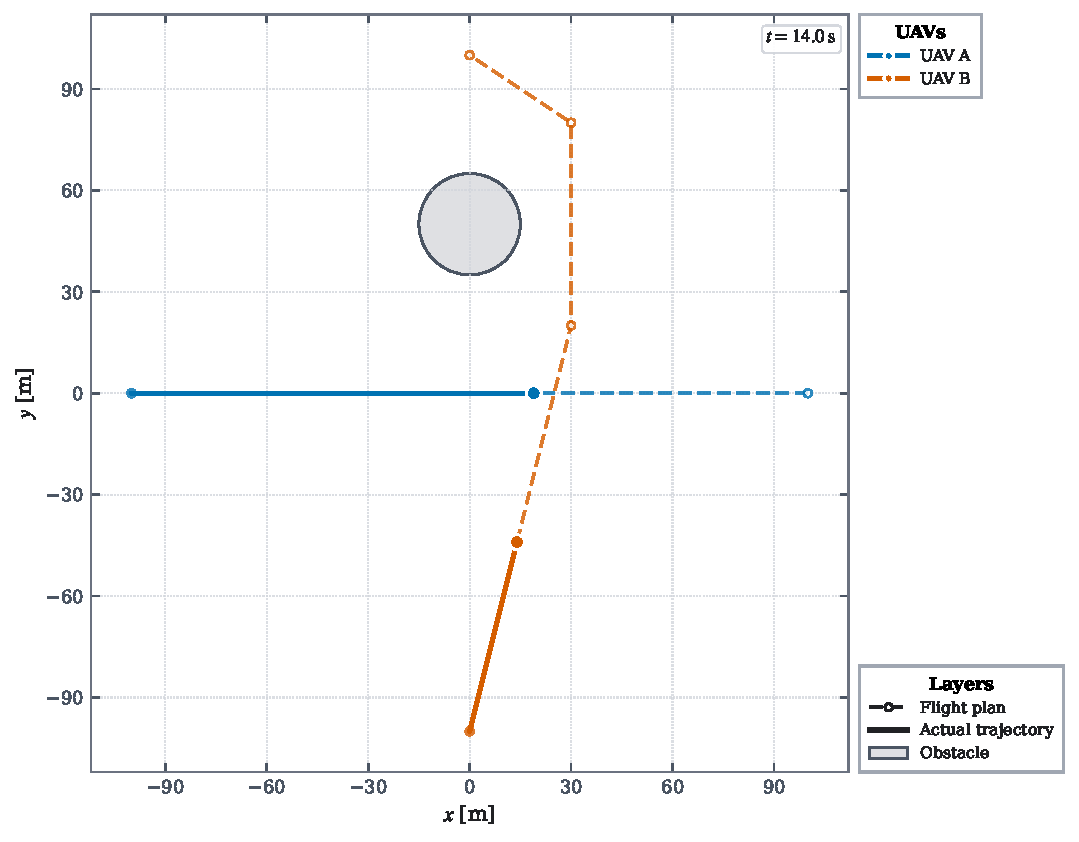
\includegraphics[width=0.78\linewidth]{figures/quickstart_xy.pdf}
  \caption{Quick-start scenario at \(t=14\)~s (\(xy\) view). Dashed lines are
  the current flight plans and solid lines the executed trajectories. UAV~B
  departed later and detours around the tower.}
  \label{fig:quickstart}
\end{figure}

\begin{tip}
\code{view} accepts \code{"3d"}, \code{"xy"}, \code{"xz"} and \code{"yz"}.
Saving to \code{.pdf} or \code{.svg} produces vector figures.
\end{tip}

% =============================================================================
\chapter{Going Further}
\label{chap:further}
% =============================================================================

\section{Tactical layer and dynamic geofences}

The tactical layer acts during flight. It needs three algorithms: a
\emph{tracking} algorithm, which predicts each UAS from its reports, a
\emph{tactical conflict predictor}, and a \emph{tactical deconfliction}
algorithm. In this new scenario a no-fly zone appears 40~m ahead of UAV~C
while it is flying, so only the tactical layer can react. The strategic
layer is disabled by omitting both strategic algorithms.

\snippet{09_tactical.py}

\snippet{10_tactical_plot.py}
\snippetoutput{10_tactical_plot.txt}

\begin{figure}[htbp]
  \centering
  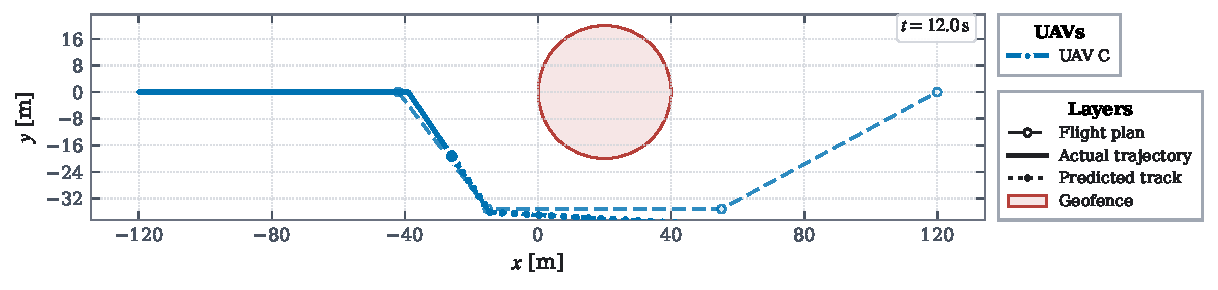
\includegraphics[width=0.92\linewidth]{figures/tactical_xy.pdf}
  \caption{Tactical detour around a geofence activated at \(t=10\)~s, shown at
  \(t=12\)~s. The dotted line is the predicted track.}
  \label{fig:tactical}
\end{figure}

\begin{note}
The tactical layer needs \code{tracking\_algorithm} and both tactical
algorithms. The prediction horizon is \code{prediction\_horizon} \(\times\)
\code{prediction\_step} seconds; a conflict can only be detected inside it.
\end{note}

\section{Plugging in your own algorithm}

Any class that inherits a contract and implements its abstract method can
replace a built-in algorithm. The strategic deconfliction contract receives
the proposal and its predicted conflicts and returns a decision, an optional
counter-proposal, and optional updates to other (inactive) plans.

\snippet{11_custom_algorithm.py}
\snippetoutput{11_custom_algorithm.txt}

Chapter~\ref{chap:custom} lists every contract and the rules each one must
follow.

\section{Reading the dataset}

\code{SimulationDataset} gives read-only access to a recorded run. Use it as a
context manager so that the SQLite connection is closed.

\snippet{12_dataset.py}
\snippetoutput{12_dataset.txt}

\section{Animations}

\snippet{13_animation.py}

\code{frame\_step} is the simulated time between frames and \code{fps} the
playback speed. Use a \code{.mp4} output path for video (requires
\code{ffmpeg}).

% =============================================================================
\chapter{Simulation Guide}
% =============================================================================

\section{Life cycle of an operation}

\begin{enumerate}[label={\color{accent}\bfseries\arabic*.}]
  \item At \code{submission\_time}, the UAS sends its proposed plan to the
    Strategic Deconfliction Module.
  \item The strategic predictor compares the proposal with the approved plans
    and the airspace snapshot; the strategic algorithm decides:
    \code{APPROVE}, \code{COUNTER\_PROPOSAL}, or \code{REJECT}.
  \item An authorized UAS waits for the time of its first waypoint and
    departs; its plan becomes \emph{active}. Strategic updates may change
    only inactive plans.
  \item In flight, the UAS sends a report every \code{report\_interval}; the
    Tracking Module produces a track for each report.
  \item Every \code{tactical\_assessment\_interval}, the tactical predictor
    checks all current tracks; the tactical algorithm may issue
    \code{FlightPlanUpdate}s, which the Flight Plan Manager sends to the UASs.
  \item The operation ends when the UAS reaches its last waypoint
    (\code{COMPLETED}) or collides (\code{COLLIDED}).
\end{enumerate}

\section{Choosing the deconfliction layers}

\begin{tabularx}{\linewidth}{@{}L{3.4cm}Y@{}}
  \toprule
  \textbf{Configuration} & \textbf{Arguments of \code{Simulation}} \\
  \midrule
  No strategic layer & Omit both strategic algorithms: every proposal is
    approved unchanged. \\
  Strategic layer & \code{strategic\_conflict\_prediction\_algorithm} and
    \code{strategic\_deconfliction\_algorithm} (always together). \\
  Tracking only & \code{tracking\_algorithm} without tactical algorithms:
    tracks are computed and recorded, but nothing reacts to them. \\
  Tactical layer & \code{tracking\_algorithm} plus both tactical
    algorithms. \\
  \bottomrule
\end{tabularx}

\section{Timing parameters}

\begin{tabularx}{\linewidth}{@{}L{5.3cm}L{1.4cm}Y@{}}
  \toprule
  \textbf{Parameter} & \textbf{Default} & \textbf{Meaning} \\
  \midrule
  \code{flight\_update\_interval} & 0.1 s & Integration step of the vehicles
    and of the collision monitor \\
  \code{trajectory\_record\_interval} & 0.2 s & Sampling of the recorded
    true states \\
  \code{report\_interval} & 0.5 s & Period of the UAS reports \\
  \code{history\_window} & 6 & Reports kept per UAS by the tracker \\
  \code{prediction\_horizon} & 10 & Number of predicted states per track \\
  \code{prediction\_step} & 0.5 s & Time between predicted states \\
  \code{tactical\_assessment\_interval} & 1.0 s & Period of the tactical
    assessments \\
  \code{network\_delay} & 0 s & Delivery delay of every message \\
  \code{collision\_distance} & 1 m & Distance below which two UASs collide \\
  \code{dataset\_flush\_interval} & 10 s & Simulated time between dataset
    writes \\
  \bottomrule
\end{tabularx}

\section{Processing time}

The arguments \code{strategic\_processing\_time},
\code{tracking\_processing\_time}, and \code{tactical\_processing\_time} accept
a \code{ProcessingTimeModel}. Its \code{calculate(**context)} returns the
simulated duration of each operation, so slow algorithms produce late
decisions. The context is a dictionary with, among others, \code{module},
\code{operation} (\code{"conflict\_prediction"}, \code{"deconfliction"}, or
\code{"tracking\_prediction"}), \code{queue\_length}, and counts such as
\code{approved\_flight\_plan\_count}, \code{track\_count}, or
\code{conflict\_count}.

\begin{pycode}
from musas.simulation import ProcessingTimeModel

class LinearDelay(ProcessingTimeModel):
    """0.05 s per track plus 0.2 s per conflict."""
    def calculate(self, **context):
        return (0.05 * context.get("track_count", 0)
                + 0.2 * context.get("conflict_count", 0))
\end{pycode}

\section{Airspace changes and disturbances}

\begin{itemize}
  \item Put permanent obstacles, and geofences or wind zones that exist from
    the start, in the initial \code{Airspace}.
  \item Use \code{schedule\_geofence} and \code{schedule\_wind\_zone} to
    activate (and optionally remove) them at given times.
  \item \code{add\_*} and \code{remove\_*} change the airspace at the current
    simulated time, for example between two calls of \code{run}.
  \item Geofences are visible to the algorithms only after their activation.
    \textbf{Wind is never given to the algorithms}: it only moves the
    vehicles, and its effect must be inferred from the reports.
\end{itemize}

\begin{pycode}
from musas.airspace import Box3D, WindZone

simulation.schedule_wind_zone(
    WindZone(wind_id="gust", velocity=(0.0, 4.0, 0.0),
             geometry=Box3D(-50, 50, -200, 200, 0, 150)),
    activation_time=20.0, removal_time=40.0,
)
\end{pycode}

\section{UAS status}

\begin{tabularx}{\linewidth}{@{}L{4.6cm}Y@{}}
  \toprule
  \textbf{\code{UAVStatus}} & \textbf{Meaning} \\
  \midrule
  \code{INACTIVE} & Registered, proposal not sent yet \\
  \code{WAITING\_FLIGHT\_PLAN} & Proposal sent, waiting for the decision \\
  \code{WAITING\_DEPARTURE} & Authorized, waiting for the departure time \\
  \code{ACTIVE} & Flying \\
  \code{COMPLETED} & Reached the last waypoint and left the airspace \\
  \code{FLIGHT\_PLAN\_REJECTED} & Proposal rejected by the strategic layer \\
  \code{COLLIDED} & Collided with another UAS or an obstacle \\
  \bottomrule
\end{tabularx}

\section{Datasets}

When \code{dataset\_path} is given, the run is written incrementally to a
SQLite file every \code{dataset\_flush\_interval}; call \code{close()} at the
end. With \code{keep\_history\_in\_memory=False}, the histories are kept only
on disk, which reduces memory use in long batches. The dataset contains:

\begin{tabularx}{\linewidth}{@{}L{4.2cm}Y@{}}
  \toprule
  \textbf{Table} & \textbf{Content} \\
  \midrule
  \code{metadata} & Configuration, user metadata, run status \\
  \code{uavs} & Final status and model names of each UAS \\
  \code{flight\_plan\_waypoints} & Proposed and authorized plan versions \\
  \code{trajectory} & Sampled true states \\
  \code{tracking\_reports}, \code{tracking\_predictions} & Reports and tracks \\
  \code{airspace\_objects}, \code{airspace\_snapshots} & Obstacles,
    geofences, wind zones, and when each one was active \\
  \code{events} & Structured events of the modules (see below) \\
  \bottomrule
\end{tabularx}

The most useful events for analysis are listed below. Filter them by name
with \code{get\_events} and read their \code{details}.

\begin{tabularx}{\linewidth}{@{}L{6.0cm}Y@{}}
  \toprule
  \textbf{Event} & \textbf{Recorded when} \\
  \midrule
  \code{STRATEGIC\_DECISION\_MADE} & A proposal is approved, counter-proposed,
    or rejected \\
  \code{FLIGHT\_PLAN\_ACTIVATED}, \code{FLIGHT\_PLAN\_COMPLETED} & A flight
    starts or ends \\
  \code{TACTICAL\_CONFLICTS\_DETECTED} & A tactical assessment finds
    conflicts \\
  \code{TACTICAL\_UPDATES\_ISSUED} & The tactical layer issues updates \\
  \code{GEOFENCE\_ACTIVATED}, \code{GEOFENCE\_REMOVED} & Dynamic geofences \\
  \code{WIND\_ZONE\_ACTIVATED}, \code{WIND\_ZONE\_REMOVED} & Dynamic wind \\
  \code{UAV\_COLLIDED} & A UAS collides \\
  \bottomrule
\end{tabularx}

\section{Metrics}
\label{sec:metrics}

\code{calculate\_metrics(dataset, minimum\_separation\_distance,
collision\_distance)} returns a dictionary with:

\begin{tabularx}{\linewidth}{@{}L{5.6cm}Y@{}}
  \toprule
  \textbf{Key} & \textbf{Meaning} \\
  \midrule
  \code{loss\_of\_separation\_events} & Entries of a pair of active UASs into
    the separation sphere \\
  \code{collision\_events} & Entries into the collision distance \\
  \code{minimum\_pairwise\_separation} & Smallest recorded distance between
    UASs [m] \\
  \code{geofence\_violations}, \code{obstacle\_violations} & Entries into
    active geofences / obstacles \\
  \code{detected\_strategic\_conflicts}, \code{detected\_tactical\_conflicts}
    & Conflicts reported by the predictors \\
  \code{flights}, \code{modified\_flights}, \code{rejected\_flights} &
    Operations, plans changed at least once, rejections \\
  \code{tactical\_interventions} & Tactical cycles that issued updates \\
  \code{average\_planned\_distance}, \code{average\_actual\_distance} &
    Mean planned / executed distance [m] \\
  \code{average\_planned\_time}, \code{average\_actual\_time} & Mean planned /
    executed flight time [s] \\
  \code{per\_uav} & Per-UAS planned and actual distance and time, and number
    of plan updates \\
  \bottomrule
\end{tabularx}

\begin{note}
Executed distance and time consider only completed flights, so a rejected or
collided operation does not appear as a shorter flight.
\end{note}

% =============================================================================
\chapter{API Reference}
% =============================================================================

This chapter documents every class and function a user needs. Types follow
the Python annotations; \code{None} defaults mean ``optional''.

% -----------------------------------------------------------------------------
\section{\texorpdfstring{\pkg{musas.simulation}}{musas.simulation}}
% -----------------------------------------------------------------------------

\begin{api}{Simulation}{class}
Assembles and coordinates one UTM simulation.
\sig{Simulation(airspace, strategic\_conflict\_prediction\_algorithm=None,
strategic\_deconfliction\_algorithm=None, tracking\_algorithm=None,
tactical\_conflict\_prediction\_algorithm=None,
tactical\_deconfliction\_algorithm=None, network\_delay=0.0, \ldots)}
\begin{params}
  \p{airspace}{Airspace}{Initial airspace: obstacles and the geofences and
    wind zones present from the start.}
  \p{strategic\_conflict\_prediction\_algorithm}{ConflictPredictionAlgorithm | None}{Strategic
    predictor; provide it together with the strategic algorithm, or omit
    both to disable the strategic layer.}
  \p{strategic\_deconfliction\_algorithm}{StrategicDeconflictionAlgorithm | None}{Strategic
    decision algorithm.}
  \p{tracking\_algorithm}{TrackingAlgorithm | None}{Track predictor;
    required by the tactical layer.}
  \p{tactical\_conflict\_prediction\_algorithm}{TacticalConflictPredictionAlgorithm | None}{Tactical
    predictor; provide it together with the tactical algorithm.}
  \p{tactical\_deconfliction\_algorithm}{TacticalDeconflictionAlgorithm | None}{Tactical
    decision algorithm.}
  \p{network\_delay}{float = 0.0}{Delivery delay of every message [s].}
  \p{message\_types\_to\_log}{Collection[MessageType] | None}{Message types
    recorded as events; by default proposals, strategic responses, flight
    start/completion, and plan updates. Use \code{()} to log none.}
  \p{flight\_update\_interval}{float = 0.1}{Integration step [s].}
  \p{trajectory\_record\_interval}{float = 0.2}{Recording step of the true
    states [s].}
  \p{report\_interval}{float = 0.5}{Period of the UAS reports [s].}
  \p{history\_window}{int = 6}{Reports kept per UAS by the Tracking Module.}
  \p{prediction\_horizon}{int = 10}{Number of predicted states per track.}
  \p{prediction\_step}{float = 0.5}{Time between predicted states [s].}
  \p{tactical\_assessment\_interval}{float = 1.0}{Period of the tactical
    assessments [s].}
  \p{collision\_distance}{float = 1.0}{Collision distance between UASs [m].}
  \p{strategic\_processing\_time, tracking\_processing\_time,
    tactical\_processing\_time}{ProcessingTimeModel}{Simulated
    processing time of each module; zero by default.}
  \p{dataset\_path}{str | Path | None}{SQLite file written during the run.}
  \p{dataset\_flush\_interval}{float = 10.0}{Simulated time between
    incremental writes [s].}
  \p{dataset\_metadata}{dict | None}{Free metadata stored with the run
    (requires \code{dataset\_path}).}
  \p{overwrite\_dataset}{bool = False}{Replace an existing file.}
  \p{keep\_history\_in\_memory}{bool = True}{Also keep histories in the
    returned result; \code{False} requires \code{dataset\_path}.}
\end{params}
\end{api}

\begin{api}{Simulation.add\_uav}{method}
\sig{add\_uav(name, flight\_plan, dynamics\_algorithm, guidance\_algorithm,
sensor\_model=None, submission\_time=0.0, waypoint\_acceptance\_radius=1.0)
-> UAV}
Registers a UAS and its proposed plan. Must be called before the first
\code{run}.
\begin{params}
  \p{name}{str}{Unique identifier.}
  \p{flight\_plan}{FlightPlan}{Proposed plan; its first waypoint is the
    initial position.}
  \p{dynamics\_algorithm}{DynamicsAlgorithm}{Vehicle response to the
    velocity command.}
  \p{guidance\_algorithm}{GuidanceAlgorithm}{Velocity command toward the
    target waypoint.}
  \p{sensor\_model}{SensorModel | None}{Measurement model of the reports;
    perfect if omitted.}
  \p{submission\_time}{float = 0.0}{When the proposal is sent [s].}
  \p{waypoint\_acceptance\_radius}{float = 1.0}{Distance at which a waypoint
    is considered reached [m].}
\end{params}
\end{api}

\begin{api}{Simulation.run}{method}
\sig{run(until: float) -> SimulationResult}
Runs or continues the simulation up to the absolute time \code{until}. It
can be called several times with increasing times.
\end{api}

\begin{api}{Simulation.close / result}{methods}
\sig{close() -> None}
Flushes and closes the dataset; the run status becomes \code{COMPLETED} if
every flight ended, or \code{STOPPED} otherwise.
\sig{result() -> SimulationResult}
Snapshot of the state and histories collected so far.
\end{api}

\begin{api}{Simulation airspace methods}{methods}
\sig{schedule\_geofence(geofence, activation\_time, removal\_time=None)}
\sig{schedule\_wind\_zone(wind\_zone, activation\_time, removal\_time=None)}
\sig{add\_geofence(geofence)\quad remove\_geofence(geofence\_id) -> Geofence}
\sig{add\_wind\_zone(wind\_zone)\quad remove\_wind\_zone(wind\_id) -> WindZone}
\code{schedule\_*} activates (and optionally removes) an object at given
simulated times; \code{add\_*}/\code{remove\_*} act at the current time.
All changes are recorded in the dataset.
\end{api}

\begin{api}{SimulationResult}{dataclass}
Data collected up to the current time, returned by \code{run}.
\begin{params}[Attributes]
  \p{time}{float}{Current simulated time.}
  \p{airspace}{Airspace}{Airspace at the end of the run.}
  \p{uavs}{dict[str, UAVSnapshot]}{Final \code{name}, \code{status},
    \code{position}, \code{velocity}, and model names of each UAS.}
  \p{proposed\_flight\_plans}{dict[str, FlightPlan]}{Original proposals.}
  \p{flight\_plan\_history}{dict[str, tuple[FlightPlan, ...]]}{Authorized
    plan versions of each UAS.}
  \p{latest\_flight\_plans}{dict[str, FlightPlan]}{(property) Latest
    strategic or tactical plan of each UAS.}
  \p{state\_history}{dict[str, list[UAVStateSample]]}{Recorded
    \code{timestamp}, \code{position}, \code{velocity}, \code{status}.}
  \p{airspace\_history}{list[AirspaceSnapshot]}{Geofences and wind zones
    present after each change.}
  \p{tracking\_reports, tracking\_predictions}{list}{Reports and tracks.}
  \p{event\_history}{list[SimulationEvent]}{Module events.}
  \p{configuration}{dict}{Parameters of the run.}
  \p{dataset\_path}{Path | None}{Dataset file, if any.}
\end{params}
\sig{save(path, metadata=None, overwrite=False) -> Path}
Writes the result to a self-contained SQLite dataset.
\end{api}

\begin{api}{SimulationDataset}{class}
Read-only access to a recorded run. Supports \code{with}.
\sig{SimulationDataset(path)\quad SimulationDataset.open(path)}
\begin{params}[Properties]
  \p{metadata}{dict}{Configuration and user metadata.}
  \p{run\_status}{str}{\code{RUNNING}, \code{COMPLETED}, \code{STOPPED},
    or \code{FAILED}.}
  \p{simulation\_time, last\_committed\_time}{float}{Final and last
    written simulated times.}
  \p{uav\_names}{tuple[str, ...]}{Registered UASs.}
\end{params}
\begin{params}[Methods]
  \p{get\_uavs()}{-> list[UAVRecord]}{Final status and model names.}
  \p{get\_trajectory(uav\_name=None, start\_time=None, end\_time=None)}{->
    list[TrajectoryRecord]}{Recorded true states, optionally filtered.}
  \p{get\_flight\_plan(uav\_name, plan\_kind="proposed", plan\_version=0)}{->
    FlightPlan | None}{A stored plan; \code{plan\_kind} is
    \code{"proposed"} or \code{"authorized"}.}
  \p{get\_flight\_plan\_versions(uav\_name, plan\_kind="authorized")}{->
    tuple[int, ...]}{Available versions.}
  \p{get\_events(event\_type=None, component=None, start\_time=None,
    end\_time=None)}{-> list[StoredEvent]}{Events with \code{timestamp},
    \code{component}, \code{event}, \code{details}.}
  \p{get\_airspace\_objects(object\_type=None)}{->
    list[AirspaceObjectRecord]}{\code{"obstacle"}, \code{"geofence"}, or
    \code{"wind\_zone"}.}
  \p{get\_tracking\_reports(uav\_name=None)}{}{Stored reports.}
  \p{get\_tracking\_predictions(uav\_name=None)}{}{Stored track states.}
  \p{get\_active\_geofence\_ids(timestamp),
    get\_active\_wind\_zone\_ids(timestamp)}{-> tuple[str, ...]}{Objects
    active at an instant.}
  \p{get\_airspace\_snapshots()}{}{When the airspace changed.}
  \p{table\_count(table)}{-> int}{Number of rows of a table.}
  \p{close()}{}{Closes the connection.}
\end{params}
\end{api}

\begin{api}{VisualizationConfig}{dataclass}
Selects what \code{plot\_dataset} and \code{animate\_dataset} draw.
\begin{params}[Fields]
  \p{view}{"3d" | "xy" | "xz" | "yz" = "3d"}{Projection.}
  \p{uav\_names}{tuple[str, ...] | None}{Subset of UASs; all if
    \code{None}.}
  \p{show\_real\_trajectories, show\_current\_positions}{bool = True}{Executed
    trajectories and current positions.}
  \p{show\_flight\_plans, show\_tracks, show\_sensor\_reports}{bool =
    False}{Current plans, predicted tracks, reports.}
  \p{show\_geofences, show\_obstacles}{bool = True}{Airspace restrictions.}
  \p{show\_wind\_zones}{bool = False}{Wind regions.}
  \p{show\_labels, show\_legend, show\_grid, show\_timestamp}{bool}{Labels
    next to the UASs (off), legend, grid, and time stamp (on).}
  \p{start\_time, end\_time}{float | None}{Time window of an animation.}
  \p{frame\_step}{float = 1.0}{Simulated time between animation frames [s].}
  \p{figure\_size}{tuple = (8.0, 5.5)}{Figure size in inches.}
  \p{title}{str | None}{Figure title.}
  \p{spatial\_unit, time\_unit}{str}{Axis and time-stamp units, e.g.
    \code{"m"}, \code{"s"}.}
\end{params}
\end{api}

\begin{api}{plot\_dataset}{function}
\sig{plot\_dataset(dataset\_path, config=None, timestamp=None,
output\_path=None, dpi=300) -> Figure}
Draws the scenario at \code{timestamp} (the last recorded time if omitted)
and optionally saves it; \code{.pdf}/\code{.svg} produce vector figures.
\end{api}

\begin{api}{animate\_dataset}{function}
\sig{animate\_dataset(dataset\_path, config=None, output\_path=None, fps=10.0,
dpi=120, repeat=True) -> FuncAnimation}
Builds an animation of the run; \code{output\_path} must end in \code{.gif} or
\code{.mp4}.
\end{api}

% -----------------------------------------------------------------------------
\section{\texorpdfstring{\pkg{musas.simulation.metrics}}{musas.simulation.metrics}}
% -----------------------------------------------------------------------------

\begin{api}{calculate\_metrics}{function}
\sig{calculate\_metrics(dataset, minimum\_separation\_distance,
collision\_distance) -> dict}
Computes the standard metrics of a \code{SimulationDataset}; the keys are
listed in Section~\ref{sec:metrics}.
\end{api}

Each metric is also available as a function of a \code{SimulationDataset}:

\begin{tabularx}{\linewidth}{@{}L{8.3cm}Y@{}}
  \toprule
  \textbf{Function} & \textbf{Returns} \\
  \midrule
  \code{number\_of\_loss\_of\_separation\_events(ds, d)} & LoS events for
    separation \code{d} \\
  \code{number\_of\_collision\_events(ds, d)} & Collision events \\
  \code{minimum\_pairwise\_separation(ds)} & Smallest distance [m] \\
  \code{number\_of\_geofence\_violations(ds)} & Geofence entries \\
  \code{number\_of\_obstacle\_violations(ds)} & Obstacle entries \\
  \code{number\_of\_detected\_strategic\_conflicts(ds)} & Strategic
    conflicts \\
  \code{number\_of\_detected\_tactical\_conflicts(ds)} & Tactical conflicts \\
  \code{number\_of\_flights(ds)} & Operations \\
  \code{number\_of\_rejected\_flights(ds)} & Rejected proposals \\
  \code{number\_of\_modified\_flights(ds)} & Plans changed at least once \\
  \code{number\_of\_tactical\_interventions(ds)} & Tactical cycles with
    updates \\
  \code{number\_of\_plan\_updates(ds, uav)} & Plan changes of one UAS \\
  \code{planned\_distance(ds, uav, plan\_kind, plan\_version)} & Length of a
    stored plan [m] \\
  \code{actual\_distance(ds, uav)}, \code{actual\_flight\_time(ds, uav)} &
    Executed distance [m] / time [s] (completed flights) \\
  \code{planned\_flight\_time(ds, uav)} & Planned duration [s] \\
  \code{average\_planned\_distance(ds)}, \code{average\_actual\_distance(ds)}
    & Mean distances [m] \\
  \code{average\_planned\_flight\_time(ds)},
    \code{average\_actual\_flight\_time(ds)} & Mean durations [s] \\
  \bottomrule
\end{tabularx}

% -----------------------------------------------------------------------------
\section{\texorpdfstring{\pkg{musas.domain}}{musas.domain}}
% -----------------------------------------------------------------------------

\begin{api}{Waypoint}{dataclass}
\sig{Waypoint(x: float, y: float, z: float, t: float)}
A 4D point: position [m] and the time at which it should be reached [s].
\code{position()} returns \code{[x, y, z]}; \code{timestamp()} returns
\code{t}.
\end{api}

\begin{api}{FlightPlan}{dataclass}
\sig{FlightPlan(waypoint\_list: list[Waypoint] = [], priority: int = 0)}
Time-ordered trajectory; the waypoints are kept sorted by time.
\code{add\_waypoint(waypoint)} inserts a waypoint. Larger \code{priority}
values have precedence, and every update must preserve the priority of the
operation.
\end{api}

\begin{api}{FlightPlanUpdate}{dataclass}
\sig{FlightPlanUpdate(uav\_name: str, flight\_plan: FlightPlan)}
A complete replacement plan for one UAS, returned by deconfliction
algorithms.
\end{api}

\begin{api}{Conflict}{base class}
Empty base class of every conflict. Predictors return instances of its
subclasses; define your own with a dataclass that inherits \code{Conflict}.
The built-in subclasses are listed in Section~\ref{sec:conflict_types}.
\end{api}

\begin{api}{TrackingReport, PredictedState, TrackPrediction}{dataclasses}
\sig{TrackingReport(uav\_name, position, velocity, timestamp, received\_at)}
\sig{PredictedState(position, velocity, timestamp)}
\sig{TrackPrediction(uav\_name, estimated\_state, predicted\_states,
generated\_at)}
A report is the measured state sent by a UAS; a track is the current
estimate followed by the predicted states.
\end{api}

\begin{api}{StrategicDecision, MessageType}{enums}
\code{StrategicDecision}: \code{APPROVE}, \code{COUNTER\_PROPOSAL},
\code{REJECT}.\par
\code{MessageType}: \code{PERIODIC\_REPORT}, \code{PROPOSAL},
\code{SD\_RESPONSE}, \code{FLIGHT\_STARTED}, \code{FLIGHT\_COMPLETED},
\code{UPDATE\_FLIGHT\_PLAN}, \code{TRACK\_UPDATE}.
\end{api}

% -----------------------------------------------------------------------------
\section{\texorpdfstring{\pkg{musas.airspace}}{musas.airspace}}
% -----------------------------------------------------------------------------

\begin{api}{Airspace}{dataclass}
\sig{Airspace(obstacles={}, geofences={}, wind\_zones={})}
Container of the airspace objects, indexed by identifier.
\begin{params}[Methods]
  \p{add\_obstacle(obstacle), remove\_obstacle(obstacle\_id)}{}{Permanent
    obstacles.}
  \p{add\_geofence(geofence), remove\_geofence(geofence\_id)}{}{Geofences.}
  \p{add\_wind\_zone(wind\_zone), remove\_wind\_zone(wind\_id)}{}{Wind
    zones.}
  \p{active\_geofences\_at(t)}{-> list[Geofence]}{Geofences active at
    \code{t}.}
  \p{wind\_at(position, t)}{-> list[float]}{Resulting wind vector.}
  \p{is\_prohibited(position, t)}{-> bool}{Inside an obstacle or active
    geofence.}
  \p{prohibited\_regions\_at(position, t)}{-> list}{Restrictions that
    contain the position.}
\end{params}
\end{api}

\begin{api}{Box3D, Cylinder3D, Geometry}{geometries}
\sig{Box3D(minimum\_x, maximum\_x, minimum\_y, maximum\_y, minimum\_z,
maximum\_z)}
\sig{Cylinder3D(center\_x, center\_y, radius, minimum\_z, maximum\_z)}
Axis-aligned box and vertical cylinder [m]. Both implement
\code{contains(position) -> bool}. A custom shape inherits \code{Geometry}
and implements \code{contains} (the built-in detour planner supports only
boxes and cylinders).
\end{api}

\begin{api}{Obstacle}{dataclass}
\sig{Obstacle(obstacle\_id, geometry, name=None)}
Permanently prohibited region; entering it is a collision.
\end{api}

\begin{api}{Geofence}{dataclass}
\sig{Geofence(geofence\_id, geometry, active\_from=None, active\_until=None,
name=None)}
KEEP\_OUT region; entering it is a violation. \code{active\_from} and
\code{active\_until} give an optional validity interval;
\code{is\_active\_at(t)} and \code{prohibits(position, t)} test it.
\end{api}

\begin{api}{WindZone}{dataclass}
\sig{WindZone(wind\_id, geometry, velocity, active\_from=None,
active\_until=None, name=None)}
Region where the constant \code{velocity} vector [m/s] is added to the
motion of the UASs. Overlapping zones add up.
\end{api}

% -----------------------------------------------------------------------------
\section{\texorpdfstring{\pkg{musas.algorithms}}{musas.algorithms}: built-in algorithms}
% -----------------------------------------------------------------------------

The built-in algorithms are simple reference implementations. They are meant
to exercise the framework and to serve as baselines, not as definitive UTM
algorithms. The contracts they implement are described in
Chapter~\ref{chap:custom}.

\subsection{Vehicle models}

\begin{api}{FirstOrderDynamics}{DynamicsAlgorithm}
\sig{FirstOrderDynamics(max\_acceleration=3.0, velocity\_time\_constant=1.0)}
The velocity follows the command with time constant
\code{velocity\_time\_constant} [s] (0 = instantaneous), limited by
\code{max\_acceleration} [m/s\textsuperscript{2}]. Wind is added to the
resulting motion.
\end{api}

\begin{api}{WaypointGuidance}{GuidanceAlgorithm}
\sig{WaypointGuidance(min\_speed=0.0, max\_speed=20.0)}
Commands the velocity that reaches the target waypoint at its scheduled
time, bounded by the speed limits [m/s].
\end{api}

\begin{api}{PerfectSensor, GaussianSensor}{SensorModel}
\sig{PerfectSensor()}
\sig{GaussianSensor(position\_standard\_deviation=1.0,
velocity\_standard\_deviation=0.1, seed=None)}
Perfect measurements, or measurements with independent zero-mean Gaussian
noise.
\end{api}

\begin{api}{ConstantTimeProcessing}{ProcessingTimeModel}
\sig{ConstantTimeProcessing(delay=0.0)}
Same processing delay [s] for every operation.
\end{api}

\subsection{Strategic layer}

\begin{api}{MinimumSeparationConflictPrediction}{ConflictPredictionAlgorithm}
\sig{MinimumSeparationConflictPrediction(minimum\_separation\_distance=30.0,
sampling\_interval=0.5, terminal\_buffer=1.0, terminal\_radius=5.0)}
Samples the proposal and each approved plan over their common time window
and reports the first traffic conflict with each UAS (distance below the
separation) and the first airspace conflict with each restriction. A
terminal rule also reports a plan that departs less than
\code{terminal\_radius} from the destination of another, at most
\code{terminal\_buffer} seconds after its arrival.
\end{api}

\begin{api}{RecursiveTimeShiftDeconfliction}{StrategicDeconflictionAlgorithm}
\sig{RecursiveTimeShiftDeconfliction(conflict\_prediction\_algorithm=None,
path\_planner=None, time\_shift\_step=5.0, maximum\_time\_shifts=20)}
Removes airspace conflicts with \code{path\_planner} and then delays the
departure in steps of \code{time\_shift\_step} until the plan is separated
from every approved plan (first-come, first-served; approved plans are never
changed). Rejects the proposal after \code{maximum\_time\_shifts}.
\end{api}

\begin{api}{DetourPathPlanner}{helper}
\sig{DetourPathPlanner(conflict\_prediction\_algorithm=None,
lateral\_clearance=10.0, vertical\_clearance=10.0, maximum\_maneuvers=4,
allow\_lateral=True, allow\_vertical=True)}
Plans a short detour around obstacles and active geofences: lateral first,
vertical as fallback. \code{plan(flight\_plan, airspace)} returns the new plan
or \code{None}.
\end{api}

\subsection{Tactical layer}

\begin{api}{FlightPlanAwareTracking}{TrackingAlgorithm}
\sig{FlightPlanAwareTracking()}
Predicts along the authorized plan, corrected by the observed position
offset and velocity error, so disturbances such as wind are carried into the
track. The track ends at the predicted arrival.
\end{api}

\begin{api}{MinimumSeparationTacticalConflictPrediction}{TacticalConflictPredictionAlgorithm}
\sig{MinimumSeparationTacticalConflictPrediction(minimum\_separation\_distance=30.0,
maximum\_time\_difference=0.5)}
Compares each pair of tracks at matching instants (within
\code{maximum\_time\_difference}) and checks every track against obstacles
and active geofences.
\end{api}

\begin{api}{HybridGeometricManeuver}{TacticalDeconflictionAlgorithm}
\sig{HybridGeometricManeuver(conflict\_prediction\_algorithm=None,
minimum\_separation\_distance=30.0, vertical\_offset=40.0,
airspace\_clearance=10.0, maneuver\_duration=5.0, recovery\_duration=8.0,
minimum\_speed=1.0, maximum\_speed=25.0, cooldown=5.0,
maximum\_escape\_distance=500.0)}
Vertical offset for traffic conflicts and lateral detour (or escape, when the
UAS is already inside) for airspace conflicts. The lower-priority UAS
maneuvers (the later one in FCFS order for equal priorities). Candidates are
validated against the other tracks and restrictions, and \code{cooldown}
limits successive maneuvers of the same UAS.
\end{api}

\begin{api}{ExtendedHybridGeometricManeuver}{TacticalDeconflictionAlgorithm}
\sig{ExtendedHybridGeometricManeuver(..., vertical\_offsets=(40.0, 60.0, 80.0),
lateral\_offsets=(45.0, 70.0), desired\_separation\_factor=1.5,
emergency\_time\_to\_conflict=6.0, ...)}
Extended variant for disturbed traffic: evaluates several vertical and
lateral candidates, targets \code{desired\_separation\_factor} times the
separation, keeps the observed drift in the candidate predictions, and
accepts only a candidate that improves the predicted separation. The other
parameters are those of \code{HybridGeometricManeuver}.
\end{api}

\subsection{Built-in conflict types}
\label{sec:conflict_types}

\begin{tabularx}{\linewidth}{@{}L{4.9cm}Y@{}}
  \toprule
  \textbf{Class} & \textbf{Fields} \\
  \midrule
  \code{StrategicTrafficConflict} & \code{timestamp}, \code{conflicting\_uav},
    \code{proposed\_position}, \code{conflicting\_position},
    \code{separation\_distance} \\
  \code{StrategicAirspaceConflict} & \code{timestamp}, \code{position},
    \code{restriction} \\
  \code{TacticalTrafficConflict} & \code{timestamp}, \code{uav\_name},
    \code{other\_uav}, \code{position}, \code{other\_position},
    \code{separation\_distance} \\
  \code{TacticalAirspaceConflict} & \code{timestamp}, \code{uav\_name},
    \code{position}, \code{restriction} \\
  \bottomrule
\end{tabularx}

% =============================================================================
\chapter{Writing Your Own Algorithms}
\label{chap:custom}
% =============================================================================

Each contract is an abstract base class with a single abstract method. To
create an algorithm, inherit the contract, implement the method, and pass an
instance to \code{Simulation} or \code{add\_uav}. All contracts are exported
by \pkg{musas.algorithms}.

{\small
\begin{tabularx}{\linewidth}{@{}L{6.3cm}L{3.8cm}Y@{}}
  \toprule
  \textbf{Contract} & \textbf{Method} & \textbf{Called} \\
  \midrule
  \code{ConflictPredictionAlgorithm} & \code{predict} & For each proposal \\
  \code{StrategicDeconflictionAlgorithm} & \code{deconflict} & After the
    strategic prediction \\
  \code{TrackingAlgorithm} & \code{predict} & For each report \\
  \code{TacticalConflictPredictionAlgorithm} & \code{predict} & Every
    tactical assessment \\
  \code{TacticalDeconflictionAlgorithm} & \code{deconflict} & When the
    assessment finds conflicts \\
  \code{GuidanceAlgorithm} & \code{calculate\_commanded\_velocity} & Every
    flight update \\
  \code{DynamicsAlgorithm} & \code{step} & Every flight update \\
  \code{SensorModel} & \code{measure} & For each report \\
  \code{ProcessingTimeModel} & \code{calculate} & Before each module
    operation \\
  \bottomrule
\end{tabularx}}

\section{Strategic contracts}

\begin{api}{ConflictPredictionAlgorithm.predict}{abstract}
\sig{predict(proposed\_flight\_plan, approved\_flight\_plans, airspace) ->
list[Conflict]}
Compares a proposal with every approved plan (\code{dict} by UAS name) and
with the airspace snapshot. Return an empty list when there is no conflict.
\end{api}

\begin{api}{StrategicDeconflictionAlgorithm.deconflict}{abstract}
\sig{deconflict(proposed\_flight\_plan, conflicts, inactive\_flight\_plans,
active\_flight\_plans, airspace) -> (StrategicDecision, FlightPlan | None,
list[FlightPlanUpdate])}
Returns the decision, the counter-proposal (only with
\code{COUNTER\_PROPOSAL}), and updates to other plans. Updates may change
only \emph{inactive} plans (approved but not departed); active plans are read
only context.
\end{api}

\section{Tactical contracts}

\begin{api}{TrackingAlgorithm.predict}{abstract}
\sig{predict(uav\_name, report\_history, flight\_plan, prediction\_start,
prediction\_horizon, prediction\_step) -> TrackPrediction}
Receives the last \code{history\_window} reports and the active plan of one
UAS; returns the estimated state at \code{prediction\_start} and
\code{prediction\_horizon} future states spaced by \code{prediction\_step}.
\end{api}

\begin{api}{TacticalConflictPredictionAlgorithm.predict}{abstract}
\sig{predict(tracks, airspace) -> list[Conflict]}
Receives the current track of every active UAS and the airspace snapshot;
each pair of UASs should be evaluated once.
\end{api}

\begin{api}{TacticalDeconflictionAlgorithm.deconflict}{abstract}
\sig{deconflict(conflicts, tracks, flight\_plans, airspace) ->
list[FlightPlanUpdate]}
Returns replacement plans for the UASs that must maneuver. A tactical plan
usually starts at the current estimated state and rejoins the original
route.
\end{api}

\section{Vehicle contracts}

\begin{api}{GuidanceAlgorithm.calculate\_commanded\_velocity}{abstract}
\sig{calculate\_commanded\_velocity(current\_position, current\_time,
target\_waypoint) -> list[float]}
\end{api}

\begin{api}{DynamicsAlgorithm.step}{abstract}
\sig{step(position, velocity, commanded\_velocity, dt) -> (new\_position,
new\_velocity)}
Advances the state by \code{dt}; wind is added by the simulation.
\end{api}

\begin{api}{SensorModel.measure}{abstract}
\sig{measure(position, velocity) -> \{"position": [...], "velocity":
[...]\}}
\end{api}

\section{Rules for every algorithm}

\begin{itemize}
  \item Do not modify the objects you receive; build new \code{FlightPlan}s.
  \item Keep the \code{priority} of the operation in every new plan; the
    framework rejects updates that change it.
  \item Return at most one \code{FlightPlanUpdate} per UAS in each call.
  \item Use only what you receive: wind is never given to the algorithms, and
    geofences appear only after their activation.
  \item Keep state in the instance if you need it (for example, a cooldown),
    and create a new instance for each simulation.
\end{itemize}

\section{Template: a tactical algorithm}

\begin{pycode}
from musas.algorithms import (TacticalConflictPredictionAlgorithm,
                              TacticalDeconflictionAlgorithm,
                              TacticalTrafficConflict)
from musas.domain import FlightPlan, FlightPlanUpdate, Waypoint


class ClimbOnConflict(TacticalDeconflictionAlgorithm):
    """The second UAS of each traffic conflict climbs 40 m for 10 s."""

    def deconflict(self, conflicts, tracks, flight_plans, airspace):
        updates = {}
        for conflict in conflicts:
            if not isinstance(conflict, TacticalTrafficConflict):
                continue
            name = conflict.other_uav
            if name in updates:
                continue
            state = tracks[name].estimated_state
            plan = flight_plans[name]
            x, y, z = state.position
            t = state.timestamp
            remaining = [w for w in plan.waypoint_list if w.t > t + 10.0]
            updates[name] = FlightPlanUpdate(name, FlightPlan(
                [Waypoint(x, y, z, t), Waypoint(x, y, z + 40.0, t + 5.0),
                 *remaining],
                priority=plan.priority,
            ))
        return list(updates.values())
\end{pycode}

% =============================================================================
\chapter{Troubleshooting}
% =============================================================================

\begin{tabularx}{\linewidth}{@{}L{5.4cm}Y@{}}
  \toprule
  \textbf{Message or symptom} & \textbf{Cause and solution} \\
  \midrule
  \code{ModuleNotFoundError: musas} & Install the package in the active
    environment (Chapter~2); in Jupyter, restart the kernel after
    \code{\%pip install}. \\
  \code{both strategic algorithms must be provided together} & Pass both
    strategic algorithms, or neither. \\
  \code{tracking\_algorithm is required for tactical deconfliction} & Add a
    tracking algorithm when using the tactical layer. \\
  \code{until must be greater than the current time} & \code{run(until)}
    takes an absolute time; use a value larger than the previous one. \\
  \code{simulation is closed} & A closed simulation cannot continue; create a
    new one. \\
  \code{simulation dataset already exists} & Pass \code{overwrite\_dataset=True} or choose
    another \code{dataset\_path}. \\
  The plot does not show a new obstacle & Figures are rebuilt from the
    dataset; run the simulation again after changing the scenario. \\
  No tactical reaction & The conflict is beyond the prediction horizon
    (\code{prediction\_horizon} \(\times\) \code{prediction\_step}) or the
    cooldown is active. \\
  MP4 export fails & Install \code{ffmpeg}, or save as \code{.gif}. \\
  \bottomrule
\end{tabularx}

\end{document}
